\section{Past: Year 2000} \label{past}
%\emph{Today is yesterday's pupil.}
%\para{We summarize what the weakness and need for extension of the traditional defect prediction approaches in 2000 (millennium).} We introduce them by following our scheme (i.e., data collection, metrics calculation, model building and model evaluation).

In order to grasp the level of accomplishments, it is necessary to look back and examine the challenges that faced the software defect prediction in the past. In particular, we look back since the year 2000, when Fenton \ea~\cite{Fenton1999TSE} published the seminal survey on software defect prediction. To enhance readability, we organize this section along the four dimensions used in Section~\ref{background}, i.e., data, metrics, modelling and performance evaluation.

%We summarize 10 needs for extension of the traditional defect prediction approaches in 2000 (millennium). We introduce them by following our scheme of Section~\ref{background} (i.e., data collection, metrics calculation, model building and model evaluation).

Figure \ref{fig:whole_picture} shows the overview of past, trends and future in defect prediction studies.

\begin{figure*}
  \centering
  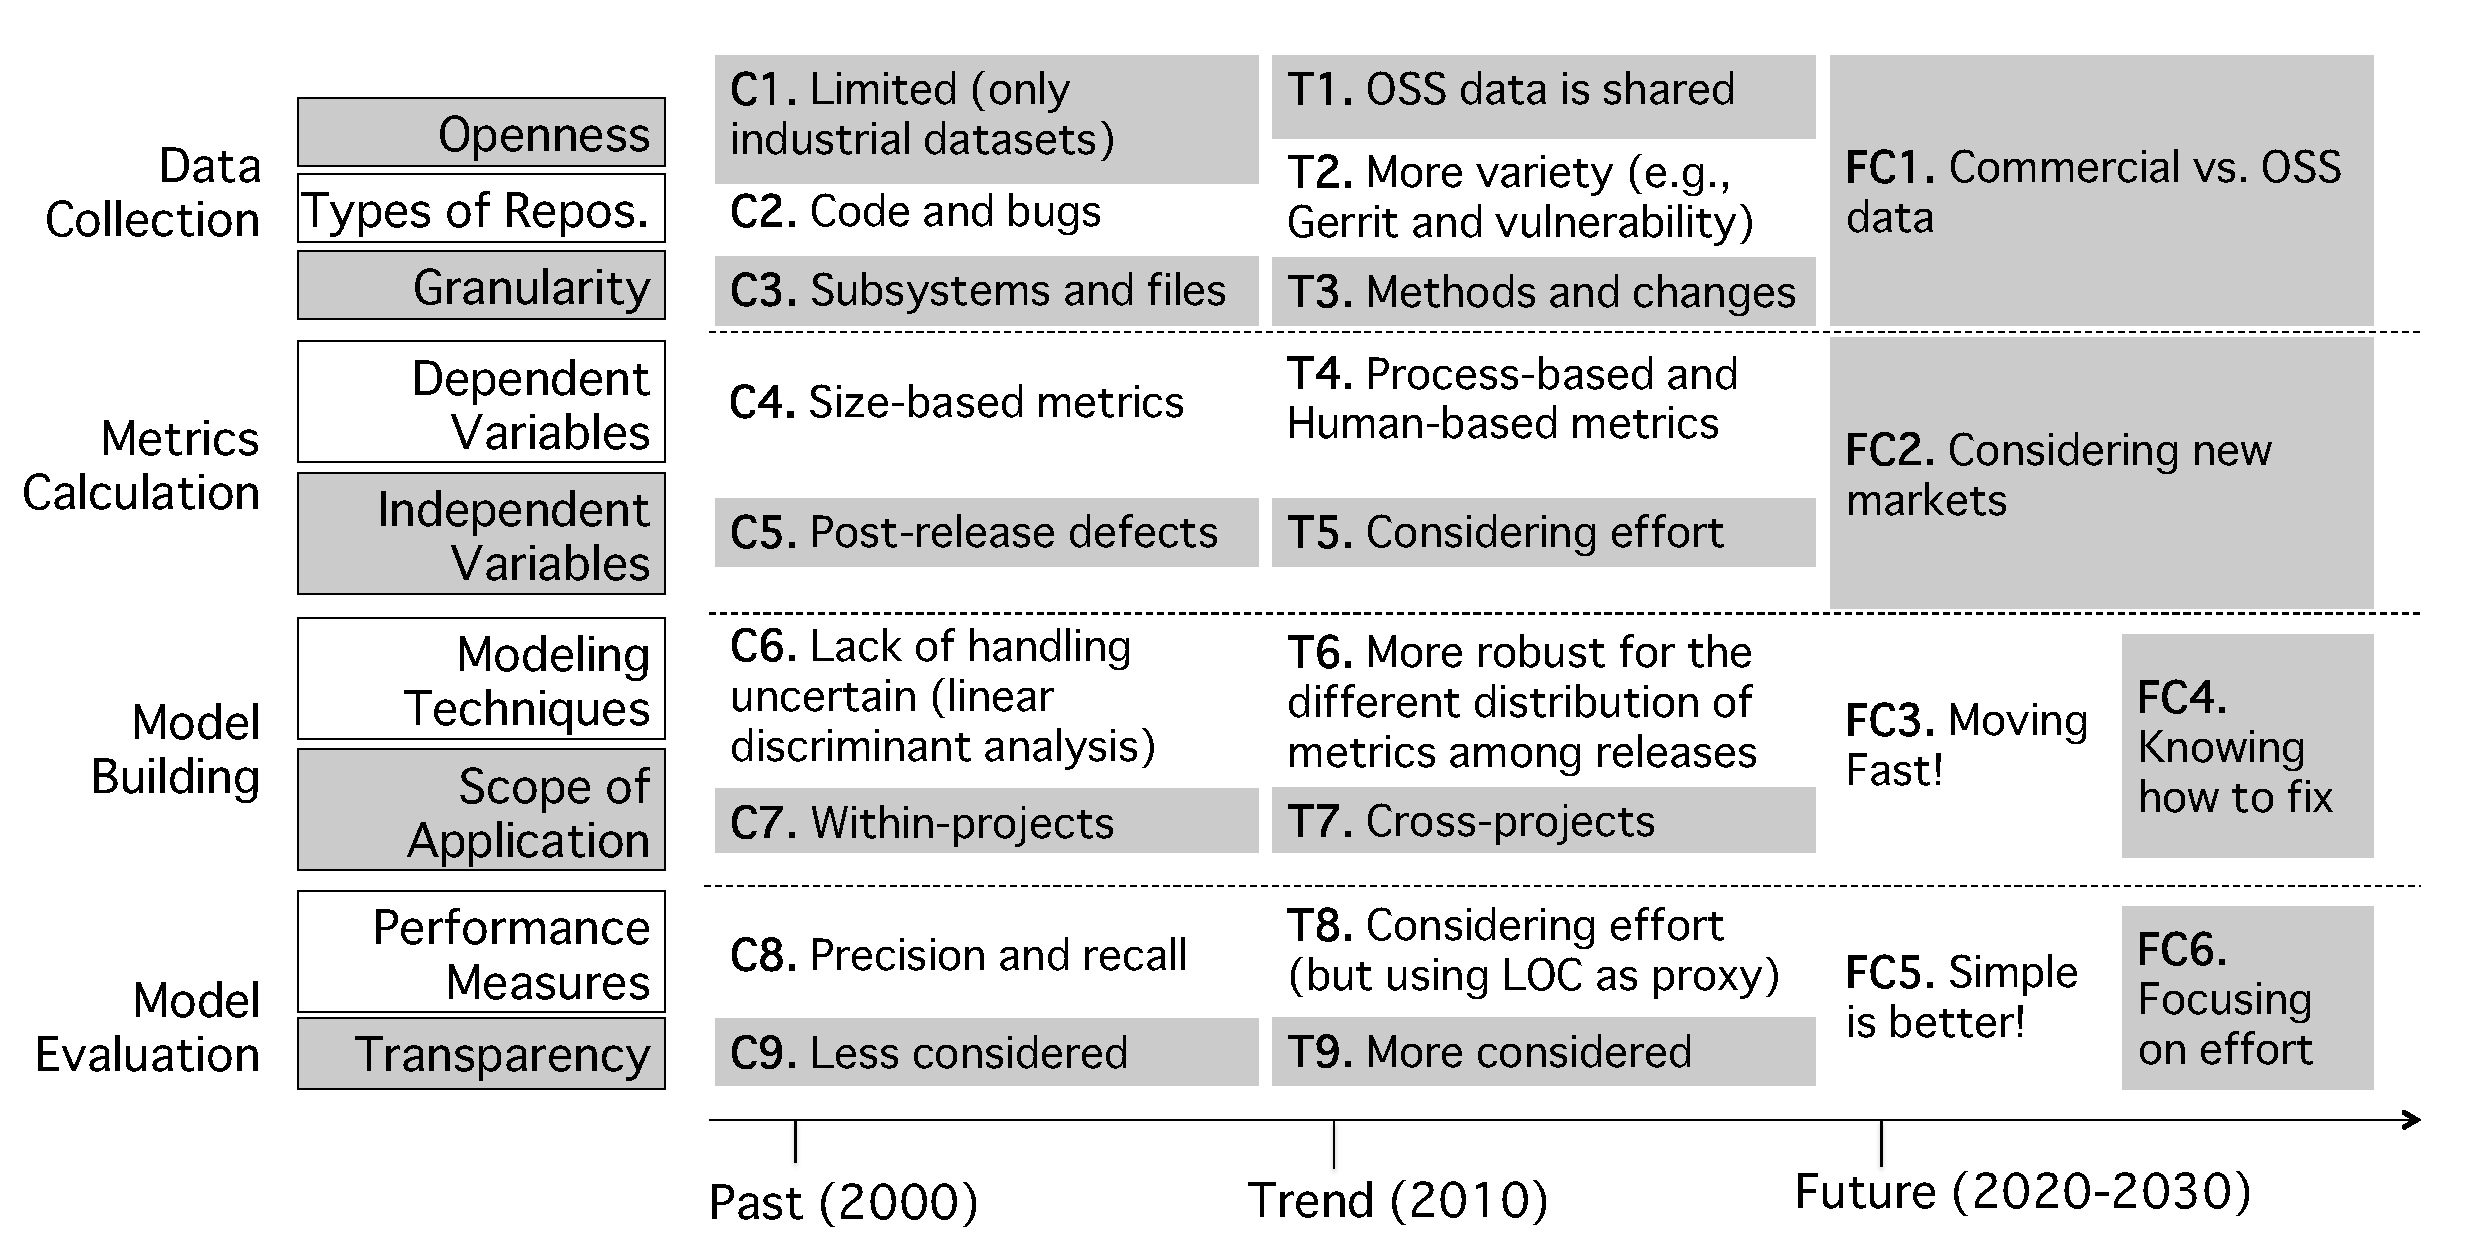
\includegraphics[width=.9\textwidth]{figures/whole_pitcture}
  \caption{Overview of Past, Trends and Future in Defect Prediction Studies \label{fig:whole_picture}}
\end{figure*}

%%%%%%%%%%%%%%%%%%%%%%%%%%%%%%%%%%%%%%%%%%%%%%%%%%%%%%%%%%%
\subsection{Data}

\smallsection{Challenge 1: Lack of Availability and Openness}
In the year 2000, one of the main challenges facing all data-driven approaches (including software defect prediction) was the lack of data availability. Software defect prediction was done only within several select, and perhaps forward-thinking, companies using their industrial data.
However, since software companies almost never want to disclose the quality of their software, researchers can never obtain the datasets used in previous studies. This was a major challenge.

Validating this challenge, a survey of software defect prediction papers published between the years 2000-2010~\cite{Shihab2012PhD} showed that 13 our of 14 defect prediction papers published between the years 2000-2002 conducted their studies using datasets collected from industrial projects. Obviously, these dataset were not shared. The other paper that used open source software data~\cite{Denaro2002ICSE}, used data from the Apache Web server project, however, they never made their datasets publicly available. This shows that back in the year 2000, data availability and openness was a real challenge facing the software defect prediction community.
% \emad{Yasu: is this what you wanted to say?}
% \yasu{Yes}

\smallsection{Challenge 2: Lack of Types of Repositories}
In addition to the lack of availability of data, the variety of the data was very limited as well. In the year 2000, most papers used data from source code and bug repositories, because those repositories provided the most basic information for building defect prediction models. For example, all 14 defect prediction studies between the years 2000 and 2002 used source code and bug repositories only~\cite{Shihab2012PhD}. Clearly, this shows that not only was data scarce, it was also very difficult to come up with different types of data.

%Nowadays, several types of repositories are available for defect prediction models, such as software review repositories (Gerrit) and vulnerability repositories. \emad{Yasu, I am not sure we should talk about what happens nowadays since we don't do that in the data collection part. What do you think?}
%\yasu{I agree}

% now we also use email, software inspection, testing.

\smallsection{Challenge 3: Lack of Variety of Granularity}
In addition to data availability and variety, the granularity of the data was another issue that faced software defect prediction work in the 2000s. The prediction unit (granularity) heavily depends on the data that is collected from the software repositories and used to build the defect prediction models. There are different levels of granularity such as the subsystem~\cite{Zimmermann2008ISSRE}, file~\cite{Dambros2010MSR} or function~\cite{Kim2007ICSE} level. 

%The finer the granularity, the better, since we will be able to narrow down the defect to a smaller code unit. Of course, the tradeoff here is that making predictions at a fine granularity is more difficult since, since for example, it is much more difficult to predict defective methods compared to subsystems, i.e., it is much easier when your unit of prediction is bigger.
%\emad{not sure if we need the last 2 sentences since the end of the next paragraph says the same thing I think}
%\yasu{I agree. I would drop the last 2 sentences.}

In 2000, the majority of studies were performed at the subsystem or file levels. Only one paper~\cite{Wong2000SPE} of the 14 defect prediction studies between 2000 and 2002 performed its prediction at the function level ~\cite{Shihab2012PhD}. The main reason for most studies performing their prediction at high levels of granularity is that repository data is often given at the file level and can be easily abstracted to the subsystem level. Although performing predictions at the subsystem and file levels may lead to better performance results~\cite{Schroter2006ISESE,Zimmermann2007}, the usefulness of the defect prediction studies becomes less significant (i.e., since more code would need to be inspected at high levels of abstraction).

%\emad{I think we should add a conclusion box here to summarize the challenges of data collection in 2000s}
%\yasu{Agree}

\conclusionbox{Software defect prediction studies in the 2000s were facing the challenges for the lack of data availability, variety and granularity.}

%%%%%%%%%%%%%%%%%%%%%%%%%%%%%%%%%%%%%%%%%%%%%%%%%%%%%%%%%%%
\subsection{Metrics}
Due to the limitations on data in the 2000s, there were several implications on the metrics and the type of metrics that were used in software defect prediction models.

\smallsection{Challenge 4: Lack of Variety of Independent Variables \textemdash Size-Based Metrics}
Size-based metrics (i.e., product metrics) are metrics that are directly related or derived from the source code (e.g., complexity or size). In the 2000s, a large body of defect prediction studies used product metrics to predict defects. The main idea behind using product metrics is that, for example, complex code is more likely to have defects. However, as Fenton and Neil mentioned~\cite{Fenton2000ICSE} in future of software engineering in 2000, while size-based metrics correlated to the number of defects, they are poor predictors of defects (i.e., there is no linearly relationship between defect density and size-based metrics). Furthermore, several studies found that code complexity metrics tend to be highly correlated with each other and with the simple measure of Lines of Code (LOC)~\cite{Fenton2000ICSE}.

%\emad{Also, we need to transition better to the post-release defects. One way would be to divide it into independent and dependent variables.}
%\yasu{I agree}

% now we use process, social, experience as metrics.

\smallsection{Challenge 5: Lack of Variety of Dependent Variables \textemdash Post-Release Defects}
Generally speaking, the majority of defect prediction studies predicted post-release defects. In fact, between 2000 and 2002, 13 of 14 defect prediction studies used post-release defects as a dependent variable~\cite{Shihab2012PhD}. Although the number of post-release defects is important and measures the quality of the released software, it is the only criteria for software quality. The fact that so many studies focused on the prediction of post-release defects is a limitation of software defect prediction work.

%\emad{same as above, we should also add a conclusion of the limitations for metrics in the 2000s.}
%\yasu{Agree}

\conclusionbox{In the 2000s, software defect prediction was focusing on size-based metrics as independent variables and post-release defects as dependent variable.}

%\smallsection{Many metrics?}

% we have some techniques to solve this problem
% http://yogi.se.rit.edu/~emad/pubs/Shihab_ESEM2010.pdf
% but is there any paper that use such 40 metrics at same time?

%%%%%%%%%%%%%%%%%%%%%%%%%%%%%%%%%%%%%%%%%%%%%%%%%%%%%%%%%%%
\subsection{Model building}
\smallsection{Challenge 6: Treating Uncertainty in Model Inputs or Outputs}
In the 2000s, linear regression and logistic regression models were often used as modeling techniques because they are simple modeling techniques. Defect prediction models assume that the distributions of the metrics in the training and testing datasets are similar~\cite{Turhan2009ESE}. However, in practice, the distribution of metrics can vary among releases. 
If the distribution vary among releases, linear regression and logistic regression models
specialize only in training data and fail prediction into testing data.

%\emad{I am not sure what you want to say here. What I would say is most use linear and logistic reg since they are simple. However, they are limited and more sophisticated techniques needed to be explored since 1) they could perform better (e.g., random forests)and 2) they may help us better understand our solutions (e.g., decision trees)}
%\yasu{What you would say is same as what I wanted to say.}

% we now have ensemble learning techniques.

\smallsection{Challenge 7: Building Models for Projects in the Initial Development Phases}
In the 2000s, most software defect prediction studies trained their models on data from the same project, usually from early releases. Then, the trained models were used to predict defects in future releases. In practice however, training data may not be available for projects in the initial development phases or for legacy systems that have not archived historical data. How to deal with projects that did not have prior project data was an open challenge in the 2000s.

%To overcome the limited availability of training data, recent work has introduced cross-project defect prediction models, i.e., models trained using historical data from other projects~\cite{Turhan2009ESE}. However, in 2000, defect prediction studies focused on only within-projects (i.e., models trained using historical data from same projects).
% \emad{I would remove this paragraph since it is not talking about the challenges man.}
% \yasu{Agree}

% we now also work on cross-projects.

%\smallsection{They are essentially black box models that hide crucial assumptions from potential users}
% decision tree or some models.

\conclusionbox{The challenges of model building in the 2000s were how to deal with projects that 
did not have the similar distributions of the metrics between training and testing datasets 
and did not have prior project data.}

%%%%%%%%%%%%%%%%%%%%%%%%%%%%%%%%%%%%%%%%%%%%%%%%%%%%%%%%%%%
\subsection{Model evaluation}

\smallsection{Challenge 8: Lack of Practical Performance Measures}
Once the prediction models are built, one of the key questions is how well do they perform. In the 2000s, many defect prediction studies empirically evaluated their performance using standard statistical measures such as precision, recall and model fit (measured in $R^2$ or deviance explained). Such standard statistical measures are fundamental criteria to know how well defect prediction models predict and explain defects. However, in some cases other more practical criteria needed to be considered. For example, how much effort is needed to address a predicted defect or the impact of a defect may need to be taken into consideration.

%  Recently, several studies try to evaluate their models using practical performance measurement.

\smallsection{Challenge 9: Lack of Transparency/Repeatability}
In the 2000s, due to the lack of availability and openness of the datasets, other studies were not able to repeat the findings of prior studies. Such lack of repeatability misses the critiques of current and new research~\cite{Shepperd2013TSE} and \cite{Ghotra2015ICSE}. Hence, comparing the performance of a technique with prior techniques was nearly impossible in the 2000s.

% Some paper shares their data and scripts to re-run their analysis.

\conclusionbox{In the 2000s, defect prediction studies were lacking the practical performance measures in industrial perspective and transparency in academic perspective.}